%%
%% This is file `sample-sigconf.tex',
%% generated with the docstrip utility.
%%
%% The original source files were:
%%
%% samples.dtx  (with options: `sigconf')
%% 
%% IMPORTANT NOTICE:
%% 
%% For the copyright see the source file.
%% 
%% Any modified versions of this file must be renamed
%% with new filenames distinct from sample-sigconf.tex.
%% 
%% For distribution of the original source see the terms
%% for copying and modification in the file samples.dtx.
%% 
%% This generated file may be distributed as long as the
%% original source files, as listed above, are part of the
%% same distribution. (The sources need not necessarily be
%% in the same archive or directory.)
%%
%% The first command in your LaTeX source must be the \documentclass command.
\documentclass[sigconf]{acmart}

%Russian-specific packages
%--------------------------------------
\usepackage[T2A]{fontenc}
\usepackage[utf8]{inputenc}
\usepackage[russian]{babel}
%--------------------------------------
 
%Hyphenation rules
%--------------------------------------
\usepackage{hyphenat}
\hyphenation{ма-те-ма-ти-ка вос-ста-нав-ли-вать}
%--------------------------------------

%% NOTE that a single column version may be required for 
%% submission and peer review. This can be done by changing
%% the \doucmentclass[...]{acmart} in this template to 
%% \documentclass[manuscript,screen]{acmart}
%% 
%% To ensure 100% compatibility, please check the white list of
%% approved LaTeX packages to be used with the Master Article Template at
%% https://www.acm.org/publications/taps/whitelist-of-latex-packages 
%% before creating your document. The white list page provides 
%% information on how to submit additional LaTeX packages for 
%% review and adoption.
%% Fonts used in the template cannot be substituted; margin 
%% adjustments are not allowed.
%%
%%
%% \BibTeX command to typeset BibTeX logo in the docs
\AtBeginDocument{%
  \providecommand\BibTeX{{%
    \normalfont B\kern-0.5em{\scshape i\kern-0.25em b}\kern-0.8em\TeX}}}

%% Rights management information.  This information is sent to you
%% when you complete the rights form.  These commands have SAMPLE
%% values in them; it is your responsibility as an author to replace
%% the commands and values with those provided to you when you
%% complete the rights form.
\setcopyright{acmcopyright}
\copyrightyear{2018}
\acmYear{2018}
\acmDOI{10.1145/1122445.1122456}

%% These commands are for a PROCEEDINGS abstract or paper.
% \acmConference[Woodstock '18]{Woodstock '18: ACM Symposium on Neural
%   Gaze Detection}{June 03--05, 2018}{Woodstock, NY}
% \acmBooktitle{Woodstock '18: ACM Symposium on Neural Gaze Detection,
%   June 03--05, 2018, Woodstock, NY}
% \acmPrice{15.00}
% \acmISBN{978-1-4503-XXXX-X/18/06}


%%
%% Submission ID.
%% Use this when submitting an article to a sponsored event. You'll
%% receive a unique submission ID from the organizers
%% of the event, and this ID should be used as the parameter to this command.
%%\acmSubmissionID{123-A56-BU3}

%%
%% The majority of ACM publications use numbered citations and
%% references.  The command \citestyle{authoryear} switches to the
%% "author year" style.
%%
%% If you are preparing content for an event
%% sponsored by ACM SIGGRAPH, you must use the "author year" style of
%% citations and references.
%% Uncommenting
%% the next command will enable that style.
%%\citestyle{acmauthoryear}

%%
%% end of the preamble, start of the body of the document source.
\begin{document}

%%
%% The "title" command has an optional parameter,
%% allowing the author to define a "short title" to be used in page headers.
\title{Super Duper Dataset for Experimental Analysis of CFPQ Algorithms}

%%
%% The "author" command and its associated commands are used to define
%% the authors and their affiliations.
%% Of note is the shared affiliation of the first two authors, and the
%% "authornote" and "authornotemark" commands
%% used to denote shared contribution to the research.
\author{Author 1}
\authornote{Both authors contributed equally to this research.}
\email{author_1@samplemail.com}
\orcid{1234-5678-9012}
\author{Author 2}
\authornotemark[1]
\email{author_2@samplemail.com}
\affiliation{%
  \institution{institution}
  \streetaddress{streetaddress}
  \city{city}
  \state{state}
  \country{country}
  \postcode{43017-6221}
}

\author{Author 3}
\email{author_3@samplemail.com}
\orcid{1234-5678-9012}
\affiliation{%
  \institution{institution}
  \streetaddress{streetaddress}
  \city{city}
  \state{state}
  \country{country}
  \postcode{43017-6221}
}

%%
%% By default, the full list of authors will be used in the page
%% headers. Often, this list is too long, and will overlap
%% other information printed in the page headers. This command allows
%% the author to define a more concise list
%% of authors' names for this purpose.
% \renewcommand{\shortauthors}{Trovato and Tobin, et al.}
%%
%% The abstract is a short summary of the work to be presented in the
%% article.
\begin{abstract}
Recently, there has been an increasing interest in solving problems related to context-free path queries (CFPQ) on graphs.
However, the development of meaningful benchmark datasets and standardized evaluation procedures is lagging, consequently hindering advancements in this area.
To solve this, we introduce the CFPQ\_Data dataset, which contains the most popular graphs for experimental analysis of CFPQ algorithms.
The collection consists of over 40 graphs of varying sizes.
We provide Python-based data loaders and implementations of the well-known CFPQ algorithms.
Here, we give an overview of the CFPQ\_Data dataset, standardized evaluation procedures, and provide baseline experiments.
All datasets are available at \href{https://github.com/JetBrains-Research/CFPQ_Data}{https://github.com/JetBrains-Research/CFPQ\_Data}.
The experiments are fully reproducible from the code available at \href{https://github.com/JetBrains-Research/CFPQ_PyAlgo}{https://github.com/JetBrains-Research/CFPQ\_PyAlgo}.
\end{abstract}

%%
%% The code below is generated by the tool at http://dl.acm.org/ccs.cfm.
%% Please copy and paste the code instead of the example below.
%%
% \begin{CCSXML}
% <ccs2012>
%  <concept>
%   <concept_id>10010520.10010553.10010562</concept_id>
%   <concept_desc>Computer systems organization~Embedded systems</concept_desc>
%   <concept_significance>500</concept_significance>
%  </concept>
%  <concept>
%   <concept_id>10010520.10010575.10010755</concept_id>
%   <concept_desc>Computer systems organization~Redundancy</concept_desc>
%   <concept_significance>300</concept_significance>
%  </concept>
%  <concept>
%   <concept_id>10010520.10010553.10010554</concept_id>
%   <concept_desc>Computer systems organization~Robotics</concept_desc>
%   <concept_significance>100</concept_significance>
%  </concept>
%  <concept>
%   <concept_id>10003033.10003083.10003095</concept_id>
%   <concept_desc>Networks~Network reliability</concept_desc>
%   <concept_significance>100</concept_significance>
%  </concept>
% </ccs2012>
% \end{CCSXML}

% \ccsdesc[500]{Computer systems organization~Embedded systems}
% \ccsdesc[300]{Computer systems organization~Redundancy}
% \ccsdesc{Computer systems organization~Robotics}
% \ccsdesc[100]{Networks~Network reliability}

%%
%% Keywords. The author(s) should pick words that accurately describe
%% the work being presented. Separate the keywords with commas.
% \keywords{datasets, neural networks, gaze detection, text tagging}

%% A "teaser" image appears between the author and affiliation
%% information and the body of the document, and typically spans the
%% page.
% \begin{teaserfigure}
%   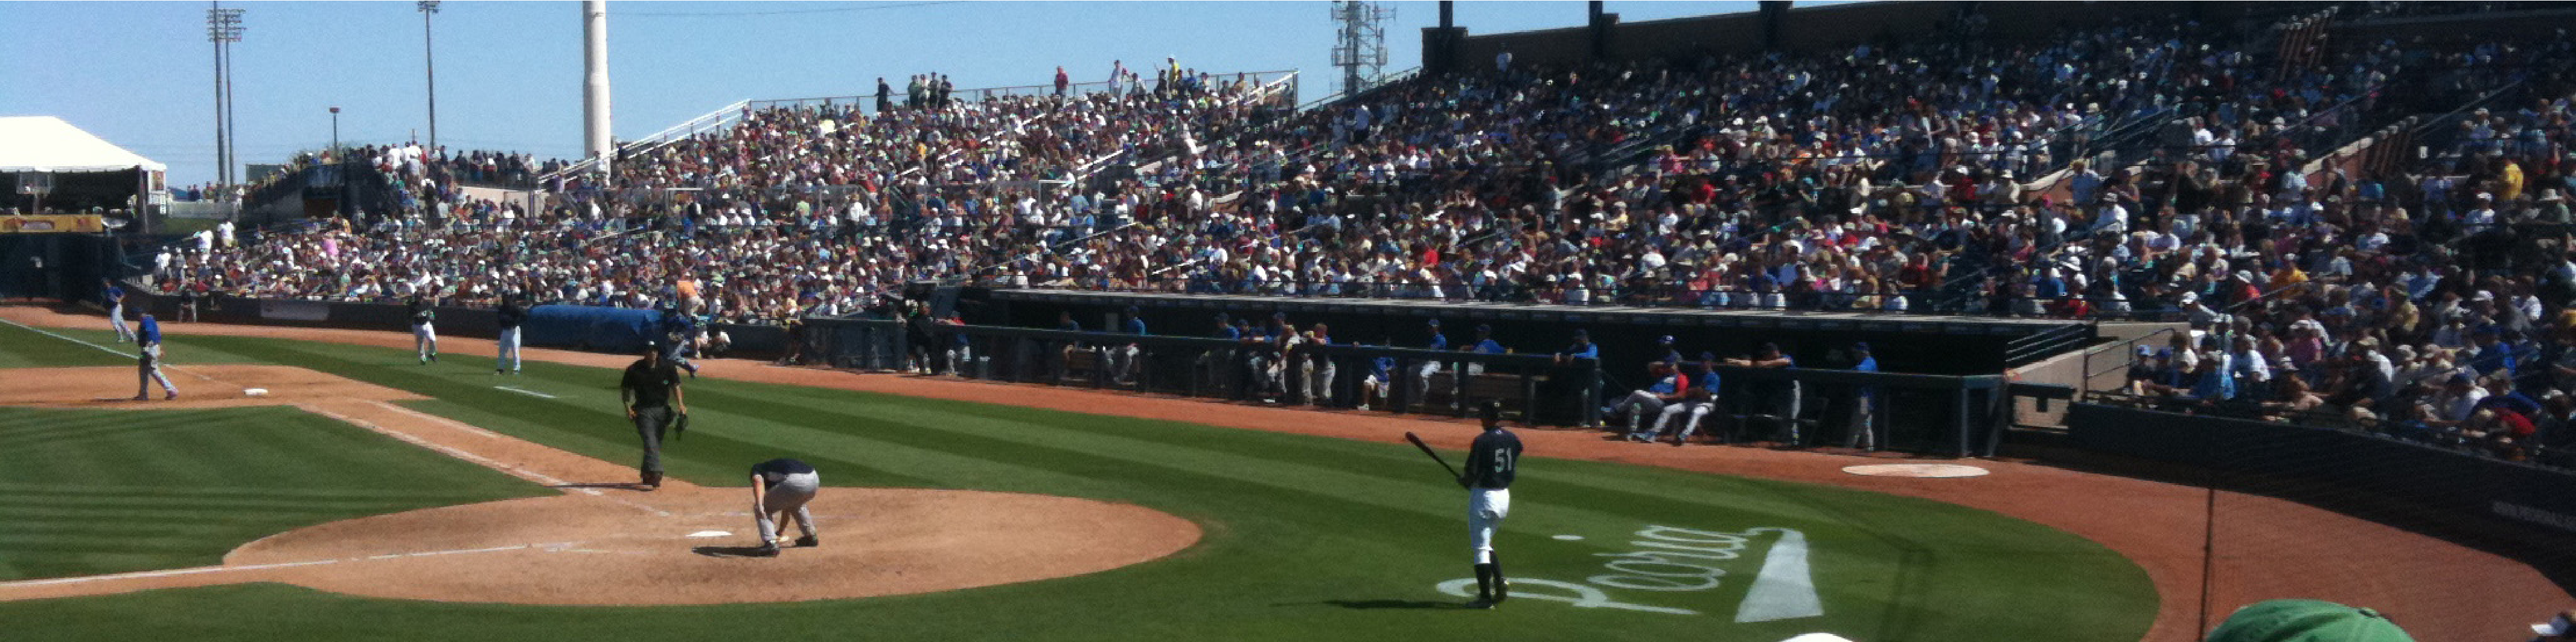
\includegraphics[width=\textwidth]{sampleteaser}
%   \caption{Seattle Mariners at Spring Training, 2010.}
%   \Description{Enjoying the baseball game from the third-base
%   seats. Ichiro Suzuki preparing to bat.}
%   \label{fig:teaser}
% \end{teaserfigure}

%%
%% This command processes the author and affiliation and title
%% information and builds the first part of the formatted document.
\maketitle

\section{Introduction}


Language-constrained path querying~\cite{barrett2000formal} is a technique for graph navigation querying.
This technique allows one to use formal languages as constraints on paths in edge-labeled graphs: path satisfies constraints if labels along it form a word from the specified language.

The utilization of regular languages as constraints, or \textit{Regular Path Querying} (RPQ), is most well-studied and widespread.
Different aspects of RPQs are actively studied in graph databases~\cite{10.1145/2463664.2465216, 10.1145/3104031,10.1145/2850413}, while regular constraints are supported in such popular query languages as PGQL~\cite{10.1145/2960414.2960421} and SPARQL\footnote{Specification of regular constraints in SPARQL property paths: \url{https://www.w3.org/TR/sparql11-property-paths/}. Access date: 07.07.2020.}~\cite{10.1007/978-3-319-25007-6_1} (property paths).
Nevertheless, there is certainly room for improvement of RPQ efficiency, and new solutions are being created~\cite{Wang2019,10.1145/2949689.2949711}.

At the same time, using more powerful languages, namely context-free languages, as constraints has gained popularity in the last few years.
\textit{Context-Free Path Querying} problem (CFPQ) was introduced by Mihalis Yannakakis in 1990 in~\cite{Yannakakis}.
Many algorithms were proposed since that time, but recently, Jochem Kuijpers et al. showed in~\cite{Kuijpers:2019:ESC:3335783.3335791} that state-of-the-art CFPQ algorithms are not performant enough for practical use.
This motivates us to develop new algorithms for CFPQ.

One promising way to achieve high-performance solutions for graph analysis problems is to reduce them to linear algebra operations.
This way, GraphBLAS~\cite{7761646} API, the description of basic linear algebra primitives, was proposed.
Solutions that use libraries that implement this API, such as SuiteSparce~\cite{10.1145/3322125} and CombBLAS~\cite{10.1177/1094342011403516}, show that reduction to linear algebra is a way to utilize high-performance parallel and distributed computations for graph analysis.

Rustam Azimov shows in~\cite{Azimov:2018:CPQ:3210259.3210264} how to reduce CFPQ to matrix multiplication.
Later, it was shown in~\cite{Mishin:2019:ECP:3327964.3328503} and~\cite{10.1145/3398682.3399163} that utilization of appropriate libraries for linear algebra for Azimov's algorithm implementation makes a practical solution for CFPQ.
However Azimov's algorithm requires transforming the input grammar to Chomsky Normal Form, which leads to the grammar size increase, and hence worsens performance, especially for regular queries and complex context-free queries.

To solve these problems, an algorithm based on automata intersection was proposed~\cite{10.1007/978-3-030-54832-2_6}.
This algorithm is based on linear algebra and does not require the transformation of the input grammar.
We improve the algorithm in this work.
We reduce the above mentioned solution to operations over Boolean matrices, thus simplifying its description and implementation.
Also, we show that this algorithm is performant enough for regular queries, so it is a good candidate for integration with real-world query languages: one algorithm can be used to evaluate both regular and context-free queries.

Moreover, we show that this algorithm opens the way to tackle a long-standing problem about the existence of truly-subcubic $O(n^{3-\epsilon})$ CFPQ algorithm ~\cite{10.1145/1328438.1328460, Yannakakis}.
Currently, the best result is an $O(n^3/\log{n})$ algorithm of Swarat Chaudhuri~\cite{10.1145/1328438.1328460}.
Also, there exist truly subcubic solutions which use fast matrix multiplication for some fixed subclasses of context-free languages~\cite{8249039}.
Unfortunately, this solutions cannot be generalized to arbitrary CFPQs.
In this work, we identify incremental transitive closure as a bottleneck on the way to achieve subcubic time complexity for CFPQ.

To sum up, we make the following contributions.
\begin{enumerate}
	\item We rethink and improve the CFPQ algorithm based on tensor-product proposed by Orachev et al. ~\cite{10.1007/978-3-030-54832-2_6}.
	We reduce this algorithm to operations over Boolean matrices.
	As a result, all-path query semantics is handled, as opposed to the previous matrix-based solution which handles only the single-path semantics.
	Also, both regular and context-free grammars can be used as queries.
	We prove the correctness and time complexity for the proposed algorithm.
	\item We demonstrate the interconnection between CFPQ and incremental transitive closure.
	We show that incremental transitive closure is a bottleneck on the way to achieve faster CFPQ algorithm for general case of arbitrary graphs as well as for special families of graphs, such as planar graphs.
	\item We implement the described algorithm and evaluate it on real-world data for both RPQ and CFPQ. Results show that the proposed solution is comparable with existing solutions for CFPQ and RPQ, thus it is a promising way to create a unified algorithm for both CFPQ and RPQ evaluation.
\end{enumerate}
\section{The CFPQ\_Data collection}
\textbf{Краткое описание того, что собрано.}
Коллекция состоит из более чем 40 графов разного размера.
Также мы предоставляем загрузчики данных и реализации наиболее популярных алгоритмов на основе Python, а также стандарт проведения экспериментов и базовых показателей работы алгоритма.
\textbf{Возможно сказать про листинг с примером кода.}
Например выложить на сайт питоновский ноутбук с примером применения.
Подробное описание каждого графа и другую документацию вы сможете найти на сайте коллекции.

\subsection{Graphs and grammars}
\textbf{Описываем коллекцию.}
Наша коллекция наборов данных охватывает графы из разных областей, предоставленные разными авторами. 
Здесь мы даем обзор некоторых репрезентативных областей и моделей графов.

\textbf{RDF.}
\textbf{Рассказать откуда взялись RDF.}
Small graphs is a set of popular semantic web ontologies. This set is introduced by Xiaowang Zhang in "Context-Free Path Queries on RDF Graphs".

\textbf{MemoryAliases.}
\textbf{Рассказать откуда взялись MemoryAliases.}
Потом еще про MemoryAliases что-то вроде MemoryAliases — real-world data for points-to analysis of C code.
First part is a dataset form Graspan tool. The original data is placed here. This part is placed in Graspan folder.
Second part is a part of dataset form "Demand-driven alias analysis for C". This part is placed in small folder.

\textbf{LUBM.}
\textbf{Рассказать почему отдельно выделили LUBM.}
LUBM - the Lehigh University Benchmark graphs.

\textbf{Synthetic.}
\textbf{Рассказать про важность синтетических графов.}
WorstCase — graphs with two cylces; the query Brackets is a grammar for the language of correct bracket sequences.
SparseGraph — graphs generated with NetworkX to emulate sparse data. The grammar provided is a variant of the same-generation query.
ScaleFree — graphs generated by using the Barab'asi-Albert model of scale-free networks. Use with grammar ** an\_bm\_cm\_dn**, which is a query for AnBmCmDn language.
FullGraph — cycle graphs, all edges are labeled with the same token. Use with A\_star queries, which produce full graph on that dataset.

\subsection{Baselines methods (GraphBuilders, GraphLoaders & GraphSavers)}
\textbf{Здесь описываем как реализовали загрузку и работу с графами и почему так.}
Любой граф их датасета можно либо построить (если он синтетический) либо загрузить с сайта коллекции (или по пути к имеющемуся в системе графу).
А с помощью GraphSaver'а можно любой граф сохранить в нужном исследователю виде.
\textbf{Возможно стоит упомянуть про грамматики.}

\subsection{Evaluation methods (Evaluators)}
\textbf{Тут надо описать каким образом происходит запуск алгоритма на графе и грамматике из коллекции.}
Возможно описать как это выглядит технически.
А также как можно написать свой алгоритм в имеющейся инфраструктуре.

\section{Experimental evaluation}
\textbf{Наша цель здесь это представить некоторый стандарт того, как можно проводить эксперименты.}
Стоит описать, стандартный путь проведения эксперимента и классические базовые показатели извлекаемые из работы алгоритма.

\subsection{Datasets}
\textbf{Здесь нужно описать какие графы мы взяли для проведения СВОЕГО эксперимента.}
Мы взяли RDF потому что это классика. 
Взяли MemoryAliases потому что они большие. 
Взяли WorstCase потому что это важный случай в теории.

\subsection{Algorithms}
\textbf{Здесь нужно описать какие мы алгоритмы использовали в СВОЕМ эксперименте.}
Думаю достаточно взять пару матричных алгоритмов и тензорный.

\subsection{Results and discussion}
\textbf{Здесь мы суммируем полученные результаты.}
Как-то описываем полученные результаты.
Возможно сравниваем их с полученными в других статьях.
Можно написать насколько это было просто провести эксперимент в имеющейся инфраструктуре.
Если код эксперимента маленький, то можно его вставить.

\begin{table}
  \caption{Таблица с результатами эксперимента}
  \label{tab:results}
  \begin{tabular}{cccc}
    \toprule
    Graph & Grammar & Algorithm & Time\\
    \midrule
    RDF&$G_1$&Tensor&$0.001$\\
    RDF&$G_1$&Tensor&$0.001$\\
    RDF&$G_1$&Tensor&$0.001$\\
    RDF&$G_1$&Tensor&$0.001$\\
  \bottomrule
\end{tabular}
\end{table}

\section{Conclusion}

Conclusion, current state, results.

Future work. Library extension up to full GraphBLAS API implementation.

LaGraph on F\# .NET.

Evaluation. Comparison with other implementations on different devices.
Manual implementation versus translation.  

Another direction of future work is Brahma.FSharp improvements. 
First of all, it is necessary to support discriminated unions to make it possible to express custom semirings such as \texttt{Min-Plus}, as presented in listing~\ref{lst_example}. 

Also, it is necessary to add high-level abstractions for asynchronous programming, and for multi-GPU programming.
Such mechanisms can be naturally expressed in F\# with native primitives for asynchronous programming.

fusion and other optimizations.
\section{Acknowledgments}
1 We thank everybody who provided datasets for the CFPQ\_Data collection.
2 We thank everybody who provided datasets for the CFPQ\_Data collection.
3 We thank everybody who provided datasets for the CFPQ\_Data collection.
4 We thank everybody who provided datasets for the CFPQ\_Data collection.

%%
%% The acknowledgments section is defined using the "acks" environment
%% (and NOT an unnumbered section). This ensures the proper
%% identification of the section in the article metadata, and the
%% consistent spelling of the heading.
% \begin{acks}
% 1 We thank everybody who provided datasets for the CFPQ\_Data collection.
% 2 We thank everybody who provided datasets for the CFPQ\_Data collection.
% 3 We thank everybody who provided datasets for the CFPQ\_Data collection.
% 4 We thank everybody who provided datasets for the CFPQ\_Data collection.
% \end{acks}

%%
%% The next two lines define the bibliography style to be used, and
%% the bibliography file.
% \bibliographystyle{ACM-Reference-Format}
% \bibliography{sample-base}

%%
%% If your work has an appendix, this is the place to put it.
% \appendix


%%
%% The next two lines define the bibliography style to be used, and
%% the bibliography file.
\bibliographystyle{ACM-Reference-Format}
\bibliography{paper}

\end{document}
\endinput
%%
%% End of file `sample-sigconf.tex'.
